\documentclass[11pt]{book}
\usepackage[spanish,es-tabla]{babel}
\usepackage[utf8]{inputenc}
\usepackage{amsmath}
\usepackage{listings}
\usepackage[usenames]{color} %seteamos el uso de nombre y color
\definecolor{gray97}{gray}{.97}%definimos nombre y color
\usepackage{textcomp}
\lstset{
	frame=Ltb,
	framerule=1pt,
	framextopmargin=5pt, %margen de arriba
	framexbottommargin=5pt, %margen de abajo
	framexleftmargin= 2pt, %separacion del margen izquierdo
	framesep=5pt,
	rulesep=0.3pt,
	backgroundcolor=\color{gray97},
	rulesepcolor=,
	tabsize=2,
	rulecolor=\color[RGB]{106, 182, 217}, %AZUL
	upquote=true,
	aboveskip={2\baselineskip}, %despues de la linea de texto
	columns=fixed,
	showstringspaces=false,
	extendedchars=true,
	breaklines=true,
	prebreak = \raisebox{0ex}[0ex][0ex]{\ensuremath{\hookleftarrow}},
	showtabs=false,
	showspaces=false,
	showstringspaces=false,
	basicstyle=\scriptsize\ttfamily\color[RGB]{39, 100, 46}, %Numeros de lineas, simbolos, puntos y coma y demas
	identifierstyle=\ttfamily\color[RGB]{56, 140, 189}, %variables
	commentstyle=\color[RGB]{62, 179, 101}, %comentarios
	stringstyle=\color[RGB]{247, 165, 42}, %impresiones
	keywordstyle=\bfseries\color[RGB]{237, 118, 150}, %funciones
	%
	numbers=left,
	numbersep=1pt, %separacion del numero
	numberstyle=\tiny,
	numberfirstline = false,
	breaklines=true,
}
\usepackage{textcomp}
\usepackage{graphicx}
\usepackage[colorinlistoftodos]{todonotes}
\usepackage{eso-pic}
\usepackage{avant}
\usepackage[top=1.8cm,bottom=1.8cm,left=2.3cm,right=2.3cm,headsep=8pt,a4paper]{geometry}
\usepackage{fancyhdr}
\pagestyle{fancy}
\fancyhf{}
%\fancyhead[LE,RO]{UNSAAC 2019-II}
%\fancyhead[RE,LO]{Ingenieria Electrónica}
%\fancyfoot[CE,CO]{\leftmark}
\fancyfoot[CO]{\thepage}
\renewcommand{\headrulewidth}{1pt}
\renewcommand{\footrulewidth}{1pt}
\usepackage{tabu}
\usepackage{array}
\usepackage{multirow}
\usepackage{amssymb}
\usepackage{makeidx}
\usepackage{wrapfig}
\usepackage{enumerate}
\usepackage{amsmath,tikz}
\usepackage{steinmetz}
\newcommand*{\horzbar}{\rule[0.05ex]{2.5ex}{0.5pt}}
\usepackage{calc}
\usepackage{dsfont}
\usepackage{enumitem}
\usepackage{subfig}

\title{
	\textsc{Universidad Nacional de San Antonio Abad del Cusco}\\
	\textbf{Compuertas Lógicas}\\
	Preinforme 1}

\author{
	\begin{tabular}{lr}
		Edison \textsc{Abado Ancco} & 145012 \\
		Roly Sandro \textsc{Gutierrez Benito} & 182967\\
	\end{tabular}
}


\begin{document}
	
\begin{titlepage}
	\newcommand{\HRule}{\rule{\linewidth}{0.5mm}} 
	\center
	\textsc{\LARGE  Universidad Nacional de San \\[0.2cm] Antonio Abad del Cusco}\\[1.5cm] 
	
\includegraphics[width=4cm]{IMAGENES/escudo}\\[1cm]
	\textsc{\Large Facultad de Ingeniería Eléctrica, \\ Electrónica, Informática y Mecánica}\\[0.5cm] 
	\textsc{\large Escuela Profesional de Ingeniería Electrónica}\\[0.5cm]
	\textsc{\Large \textbf{Antenas}}\\[0.5cm] 
	\HRule \\[0.4cm]
	{ \huge \bfseries Cuarto Trabajo práctico}\\[0.4cm] 
	\HRule \\[1.5cm]
	\begin{minipage}{\textwidth}
		\center 
		
		\emph{Profesor:} \\
		Ing. Milton \textsc{Velasquez Curo} \\[1cm]
		
		\begin{tabular}{ll}
			\emph{Alumno:} & \emph{Código:}\\
			Edison \textsc{Abado Ancco} & 145012 \\
		\end{tabular}
	\end{minipage}\\[2cm]
	\today
\end{titlepage}


\newpage

%\tableofcontents indice bloqueado xD

\chapter{Antena con 7 elementos de fuentes independientes dependientes de coeficientes homogeneos, distribución triangular y binómico con un espaciado de $\lambda/2$}

\newpage

\section{Distribución de coeficientes homogeneo para un espaciado de \boldmath$\lambda/2$}

\noindent Definimos la simulación de las imágenes desde \eqref{a11} hasta \eqref{a15} con los siguientes parámetros:

\begin{align*}
	L =			& \ \lambda/2 = 0.5m \\
	a =			& \ 0.1mm \\
	espaciado = & \ \lambda / 2 = 0.5m \\
	f =			& \ 300MHz
\end{align*}

\noindent Usamos los coeficientes homogeneos de:
\begin{table}[!ht]
	\centering
	\begin{tabular}{c|c|c|c|c|c|c}
		$a_0$ & $a_1$ & $a_2$ & $a_3$ & $a_4$ & $a_5$ & $a_6$ \\ \hline
		1 & 1 & 1 & 1 & 1 & 1 & 1 \\
	\end{tabular}
	\caption{Coeficientes homogéneos}
	\label{tab:1}
\end{table}

\noindent Para \boldmath{$f=300MHz$} se obtiene un coeficiente de reflexión de \boldmath{$-10.908dB$} y un SWR de \boldmath{$1.796$}. 

\begin{figure}[h]
	\centering
	\subfloat[]{
		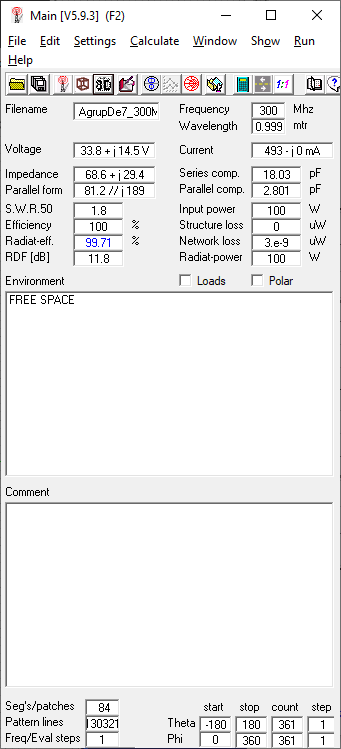
\includegraphics[scale=0.30]{IMAGENES/a11}\label{a11}}
	\subfloat[]{
		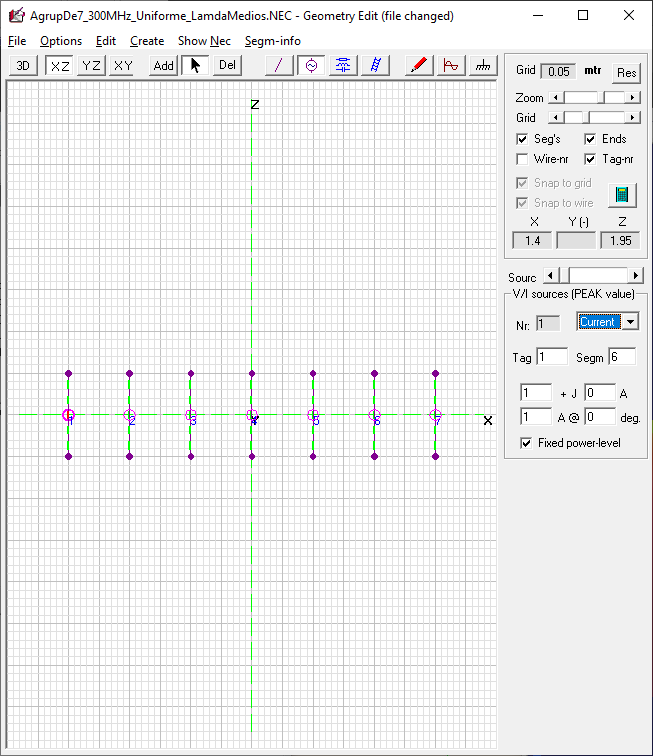
\includegraphics[scale=0.30]{IMAGENES/a12}\label{a12}}	
	\subfloat[]{
		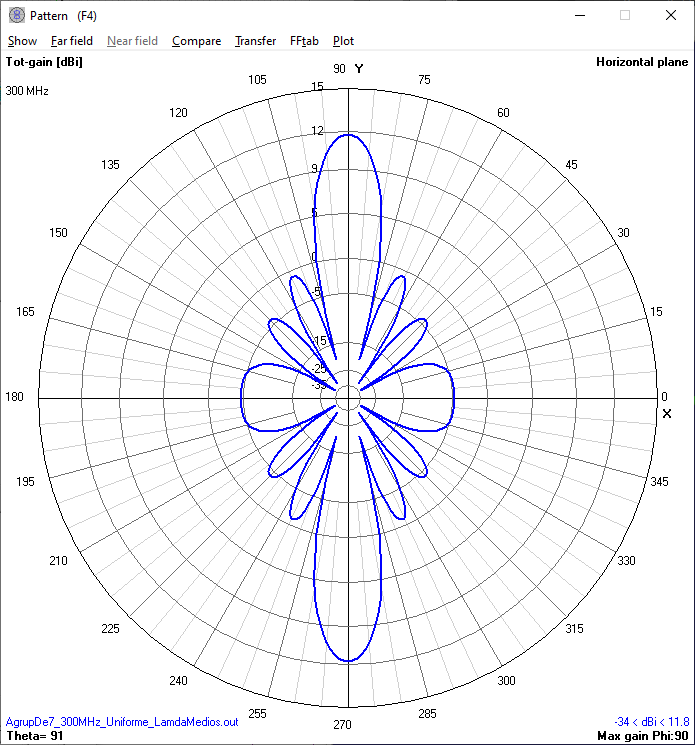
\includegraphics[scale=0.30]{IMAGENES/a13}\label{a13}} \\
	\subfloat[]{
		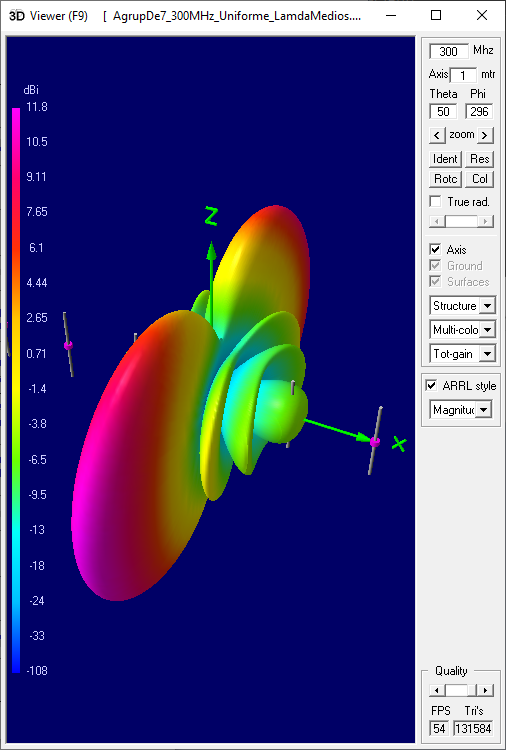
\includegraphics[scale=0.30]{IMAGENES/a14}\label{a14}}
	\subfloat[]{
		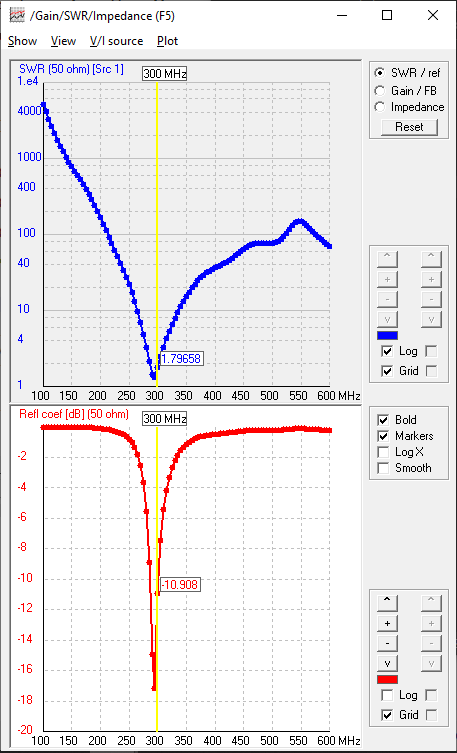
\includegraphics[scale=0.30]{IMAGENES/a15}\label{a15}}
	\caption{(a) Ventana principal para 300MHz, espaciado de $\lambda / 2$ y coeficientes homogeneos. (b) Ventana de edición para ingresar las fuentes homogeneas de acuerdo a los coeficientes. (c) Plano vertical con patrón de radiación. (d) Vista en 3D del patrón de radiación. (e)SWR y coeficiente de refleción.}
\end{figure}

\newpage
\section{Distribución de coeficientes triangular para un espaciado de \boldmath{$\lambda/2$}}

Definimos la simulación de las imágenes desde \eqref{a21} hasta \eqref{a25} con los siguientes parámetros:

\begin{align*}
	L = &\lambda/2 =  0.5m \\
	a = & 0.1mm \\
	espaciado = & \lambda / 2 = 0.5m \\
	f = & 300MHz
\end{align*}

Usamos los coeficientes homogeneos de:
\begin{table}[!ht]
	\centering
	\begin{tabular}{c|c|c|c|c|c|c}
		$a_0$ & $a_1$ & $a_2$ & $a_3$ & $a_4$ & $a_5$ & $a_6$ \\ \hline
		1 & 2 & 3 & 4 & 3 & 2 & 1 \\
	\end{tabular}
	\caption{Coeficientes homogéneos}
	\label{tab:2}
\end{table}

\noindent Para $f=300MHz$ se obtiene un coeficiente de reflexión de $-20.05dB$ y un SWR de $1.220$. 

\begin{figure}[h]
	\centering
	\subfloat[]{
		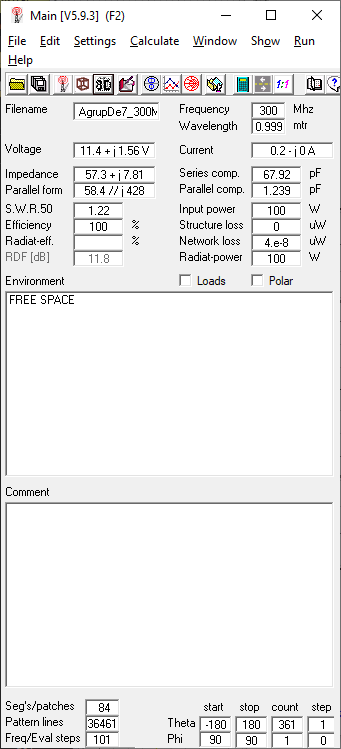
\includegraphics[scale=0.30]{IMAGENES/a21}\label{a21}}
	\subfloat[]{
		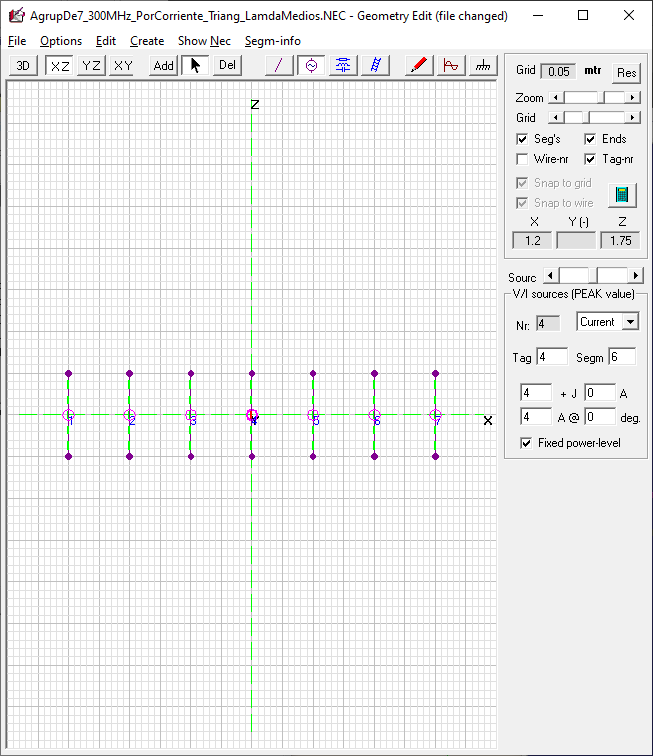
\includegraphics[scale=0.30]{IMAGENES/a22}\label{a22}}	
	\subfloat[]{
		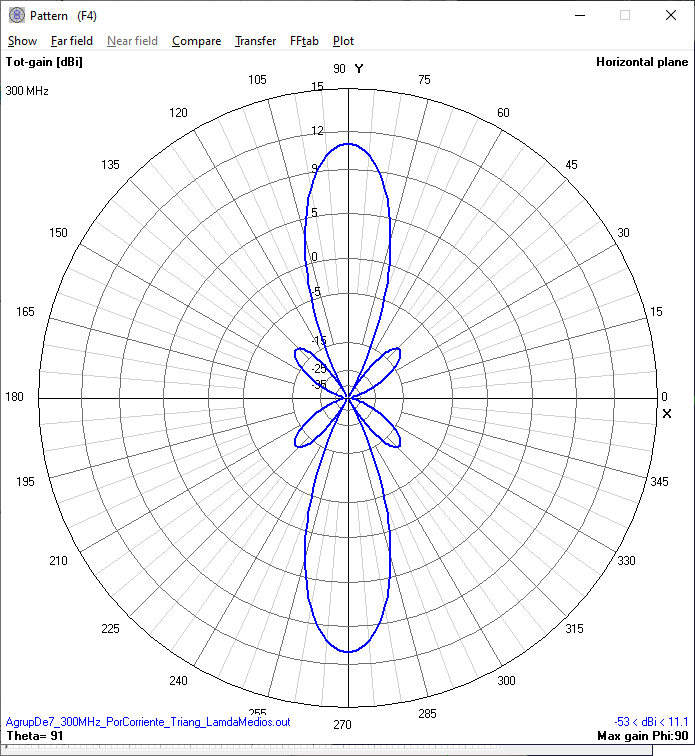
\includegraphics[scale=0.30]{IMAGENES/a23}\label{a23}} \\
	\subfloat[]{
		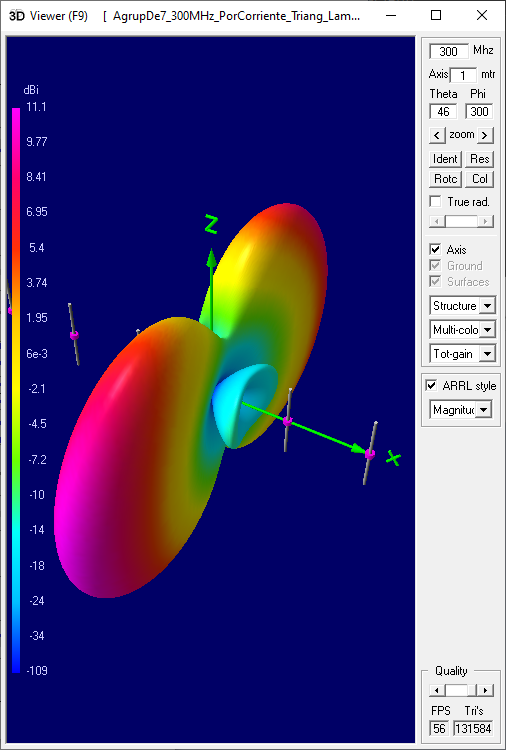
\includegraphics[scale=0.30]{IMAGENES/a24}\label{a24}}
	\subfloat[]{
		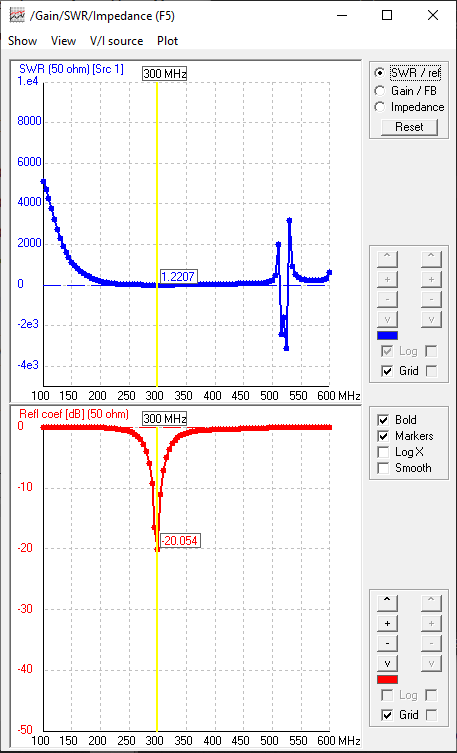
\includegraphics[scale=0.30]{IMAGENES/a25}\label{a25}}
	\caption{(a) Ventana principal para 300MHz, espaciado de $\lambda / 2$ y coeficientes homogeneos. (b) Ventana de edición para ingresar las fuentes homogeneas de acuerdo a los coeficientes. (c) Plano vertical con patrón de radiación. (d) Vista en 3D del patrón de radiación. (e)SWR y coeficiente de refleción.}
\end{figure}


\newpage
\section{Distribución de coeficientes binómico para un espaciado de $\lambda/2$}

Definimos la simulación de las imágenes desde \eqref{a31} hasta \eqref{a35} con los siguientes parámetros:

\begin{align*}
	L = &\lambda/2 =  0.5m \\
	a = & 0.1mm \\
	espaciado = & \lambda / 2 = 0.5m \\
	f = & 300MHz
\end{align*}

Usamos los coeficientes homogeneos de:
\begin{table}[!ht]
	\centering
	\begin{tabular}{c|c|c|c|c|c|c}
		$a_0$ & $a_1$ & $a_2$ & $a_3$ & $a_4$ & $a_5$ & $a_6$ \\ \hline
		1 & 6 & 15 & 20 & 15 & 6 & 1 \\
	\end{tabular}
	\caption{Coeficientes homogéneos}
	\label{tab:3}
\end{table}

Para $f=300MHz$ se obtiene un coeficiente de reflexión de $-3.184dB$ y un SWR de $5.17$. 

\begin{figure}[h]
	\centering
	\subfloat[]{
		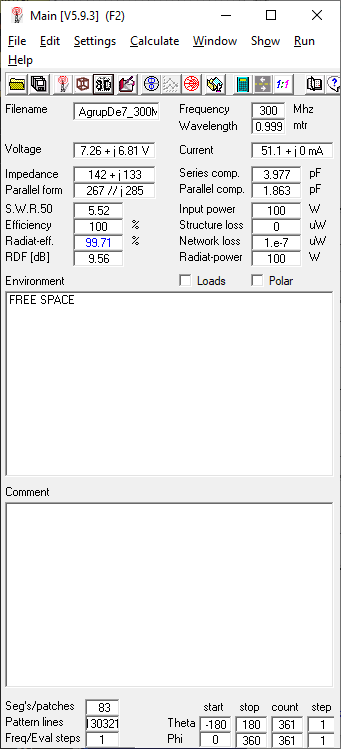
\includegraphics[scale=0.30]{IMAGENES/a31}\label{a31}}
	\subfloat[]{
		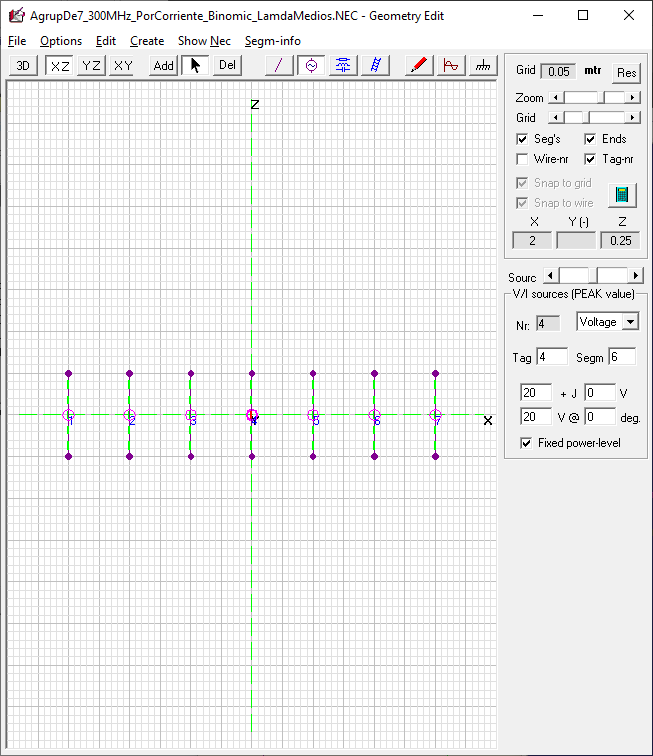
\includegraphics[scale=0.30]{IMAGENES/a32}\label{a32}}	
	\subfloat[]{
		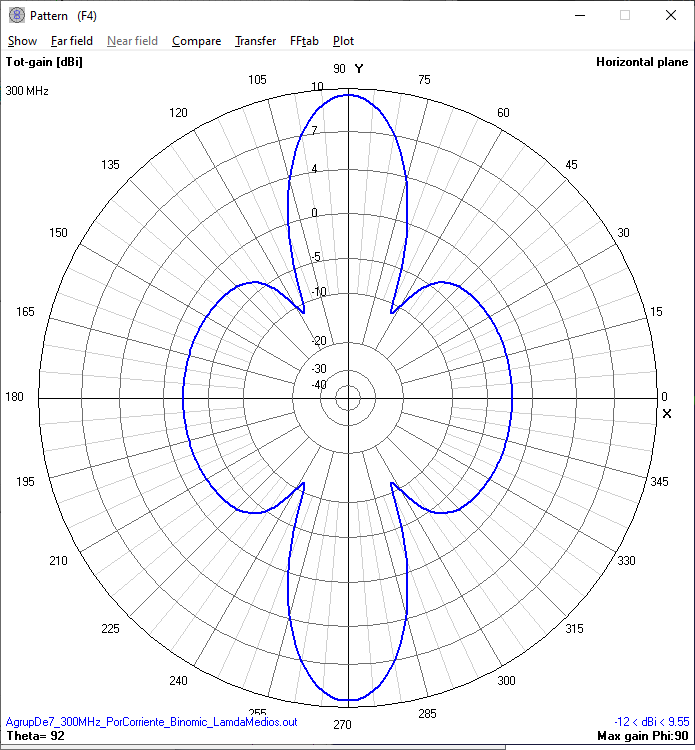
\includegraphics[scale=0.30]{IMAGENES/a33}\label{a33}} \\
	\subfloat[]{
		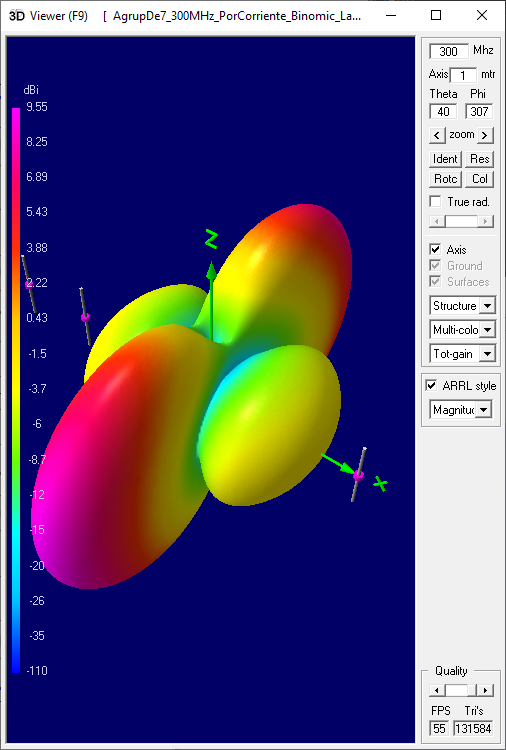
\includegraphics[scale=0.30]{IMAGENES/a34}\label{a34}}
	\subfloat[]{
		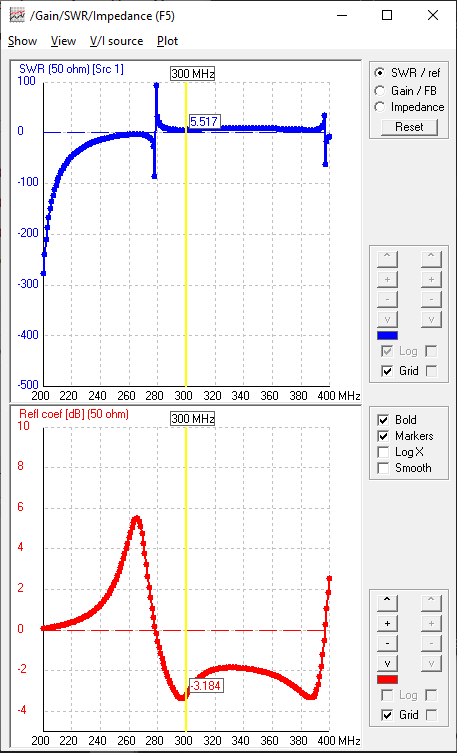
\includegraphics[scale=0.30]{IMAGENES/a35}\label{a35}}
	\caption{(a) Ventana principal para 300MHz, espaciado de $\lambda / 2$ y coeficientes homogeneos. (b) Ventana de edición para ingresar las fuentes homogeneas de acuerdo a los coeficientes. (c) Plano vertical con patrón de radiación. (d) Vista en 3D del patrón de radiación. (e)SWR y coeficiente de refleción.}
\end{figure}
\newpage


\section{Comparación de distribución de coeficientes para un espaciado de $\lambda/2$}

\begin{figure}[h]
	\centering
	\subfloat[]{
		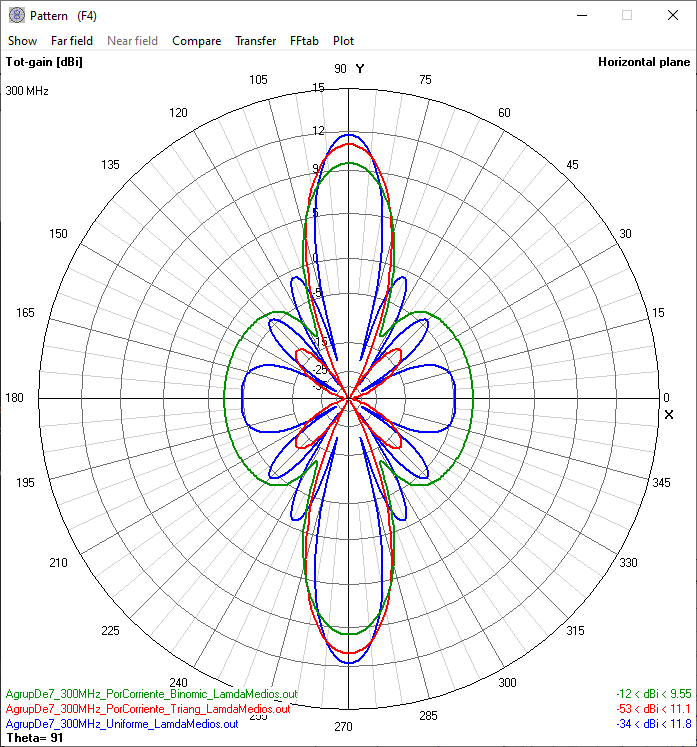
\includegraphics[scale=0.35]{IMAGENES/a111}\label{a111}}
	\subfloat[]{
		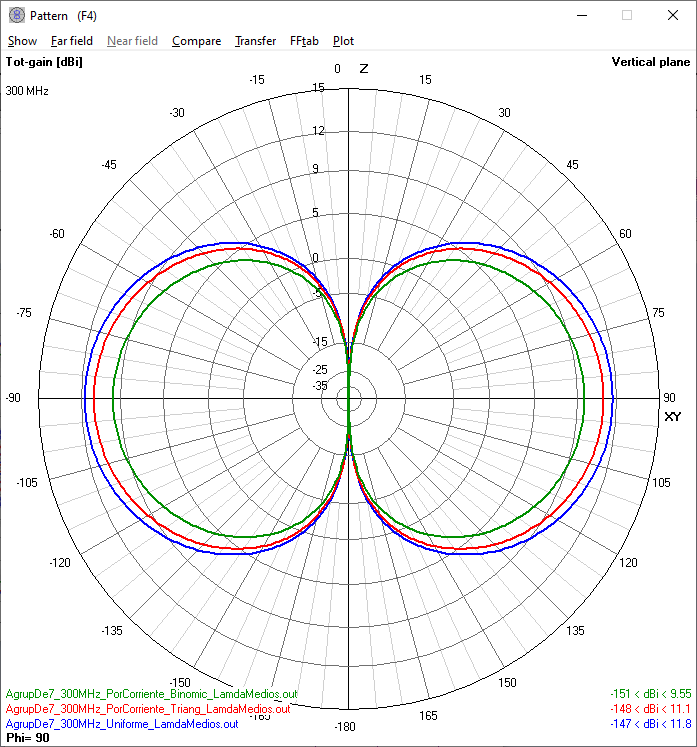
\includegraphics[scale=0.35]{IMAGENES/a222}\label{a222}}	
	\caption{(a) Patrón de radiación horizontal para 300MHz, espaciado de
	 $\lambda / 2$. (b) Patrón de radiación vertical  para 300MHz, espaciado de $\lambda / 2$.  }
\end{figure}

De las comparaciones mmostradas en las figuras podemos ver que el más ineficiente en directividad es el que tiene la distribución binomica, por lo menos para $f=300MHz$ y un $L=0.5$, la distribución binómica genera más pérdidas por que sus lóbulos secundarios crecen a pesar de que en número disminuyen.


Para hacen un enlace, se tiene que considerar en coeficeinte de acoplamiento y el SWR, el cual, con menos arreglos podemos llegar a un correcto funcionamiento con los coeficientes hallados por distribución triangular. A pesar de que tenemos menos directividad que con los coeficientes homogeneos, tenemos menos lóbulos, lo que representa menos pérdida en potencia. Además de que tenemos una impedancia de $Z = 57.3 + j7.81$, y un SWR adecuado de 1.22. Haciendo unos areglos de longitud de $L$ , radio $a$ y ligeros cambios de separación entre elementos, podemos llegar a un optimo dise;o para su correcto funcionamiento. Llegamos a $11.1dBi$, el cual podemos optimizar y mejorar.

\newpage


\chapter{Antena con 7 elementos de fuentes independientes dependientes de coeficientes homogeneos, distribución triangular y binómico con un espaciado de $\lambda/4$}

\newpage

\section{Distribución de coeficientes triangular para un espaciado de $\lambda/4$}

Definimos la simulación de las imágenes desde \eqref{a41} hasta \eqref{a45} con los siguientes parámetros:

\begin{align*}
	L = &\lambda/2 =  0.5m \\
	a = & 0.1mm \\
	espaciado = & \lambda / 4 = 0.25m \\
	f = & 300MHz
\end{align*}

Usamos los coeficientes homogeneos de:
\begin{table}[!ht]
	\centering
	\begin{tabular}{c|c|c|c|c|c|c}
		$a_0$ & $a_1$ & $a_2$ & $a_3$ & $a_4$ & $a_5$ & $a_6$ \\ \hline
		1 & 1 & 1 & 1 & 1 & 1 & 1 \\
	\end{tabular}
	\caption{Coeficientes homogénes}
	\label{tab:4}
\end{table}

Para $f=300MHz$ se obtiene un coeficiente de reflexión de $-9.60dB$ y un SWR de $1.98$. 

\begin{figure}[h]
	\centering
	\subfloat[]{
		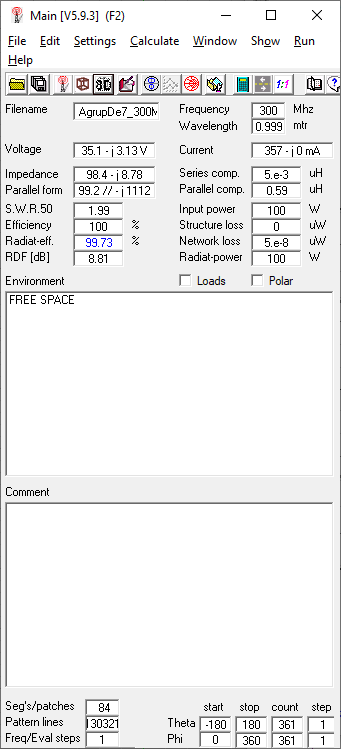
\includegraphics[scale=0.30]{IMAGENES/a41}\label{a41}}
	\subfloat[]{
		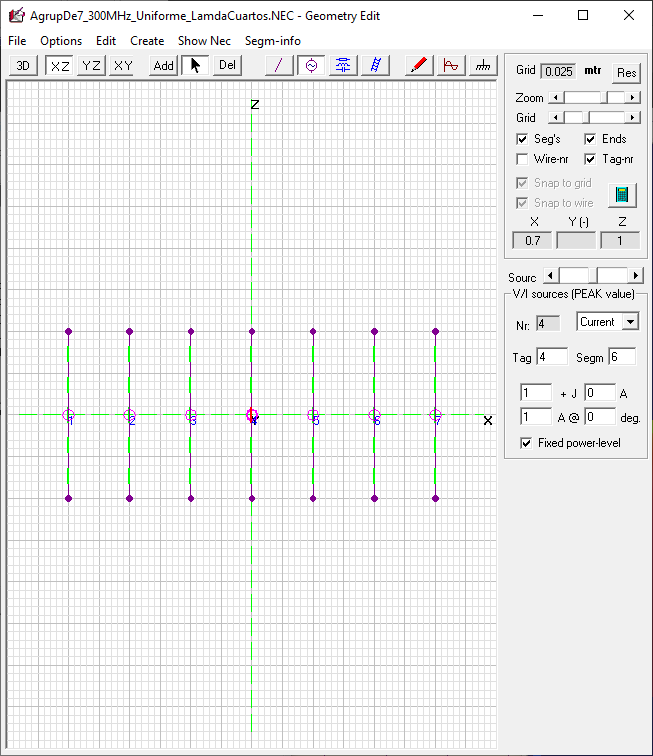
\includegraphics[scale=0.30]{IMAGENES/a42}\label{a42}}	
	\subfloat[]{
		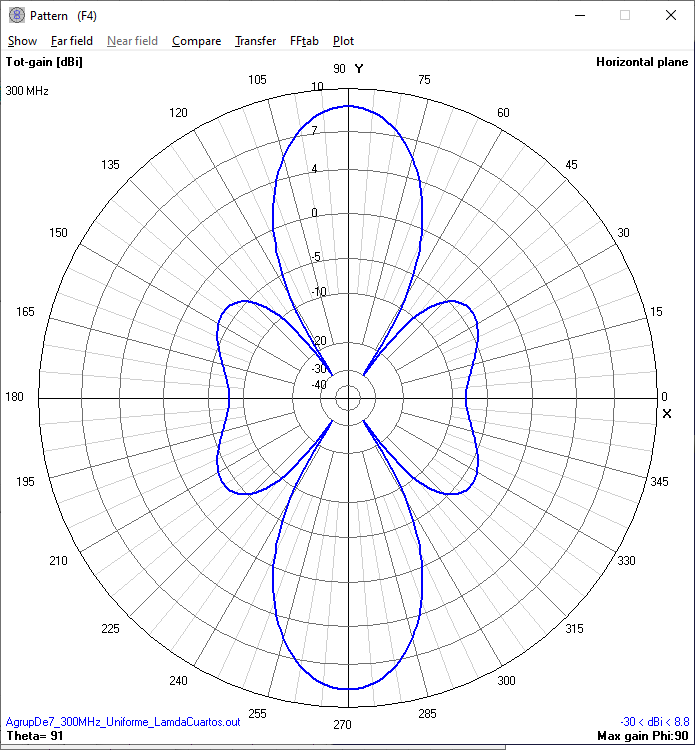
\includegraphics[scale=0.30]{IMAGENES/a43}\label{a43}} \\
	\subfloat[]{
		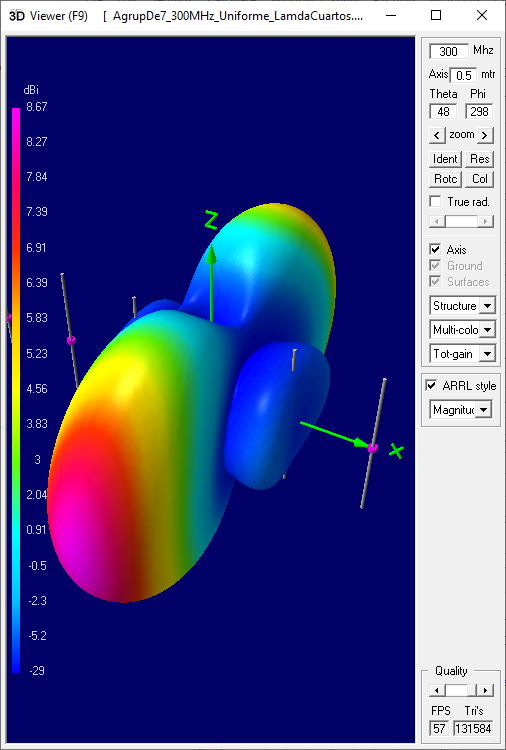
\includegraphics[scale=0.30]{IMAGENES/a44}\label{a44}}
	\subfloat[]{
		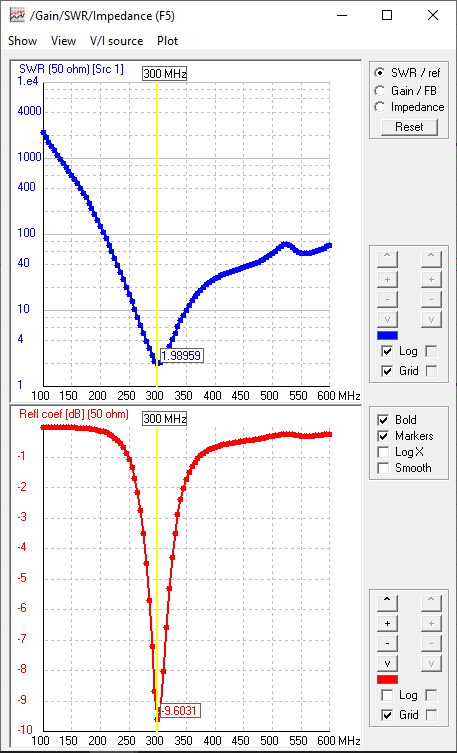
\includegraphics[scale=0.30]{IMAGENES/a45}\label{a45}}
	\caption{(a) Ventana principal para 300MHz, espaciado de $\lambda / 4$ y coeficientes homogeneos. (b) Ventana de edición para ingresar las fuentes homogeneas de acuerdo a los coeficientes. (c) Plano vertical con patrón de radiación. (d) Vista en 3D del patrón de radiación. (e)SWR y coeficiente de refleción.}
\end{figure}
\newpage

\section{Distribución de coeficientes triangular para un espaciado de $\lambda/4$}

Definimos la simulación de las imágenes desde \eqref{a51} hasta \eqref{a55} con los siguientes parámetros:

\begin{align*}
	L = &\lambda/2 =  0.5m \\
	a = & 0.1mm \\
	espaciado = & \lambda / 4 = 0.25m \\
	f = & 300MHz
\end{align*}

Usamos los coeficientes homogeneos de:
\begin{table}[!ht]
	\centering
	\begin{tabular}{c|c|c|c|c|c|c}
		$a_0$ & $a_1$ & $a_2$ & $a_3$ & $a_4$ & $a_5$ & $a_6$ \\ \hline
		1 & 2 & 3 & 4 & 3 & 2 & 1 \\
	\end{tabular}
	\caption{Coeficientes homongéneos}
	\label{tab:5}
\end{table}

Para $f=300MHz$ se obtiene un coeficiente de reflexión de $-10.908dB$ y un SWR de $1.796$. 

\begin{figure}[h]
	\centering
	\subfloat[]{
		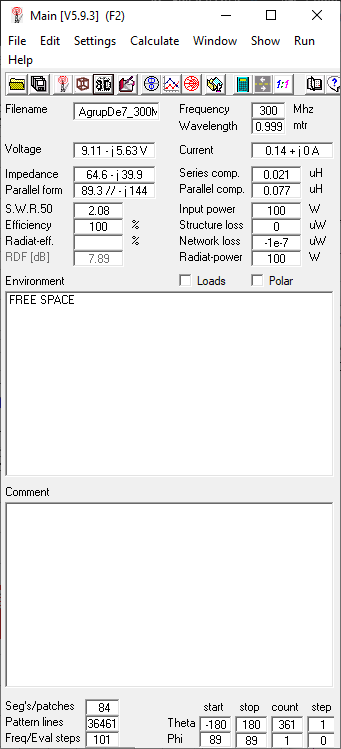
\includegraphics[scale=0.30]{IMAGENES/a51}\label{a51}}
	\subfloat[]{
		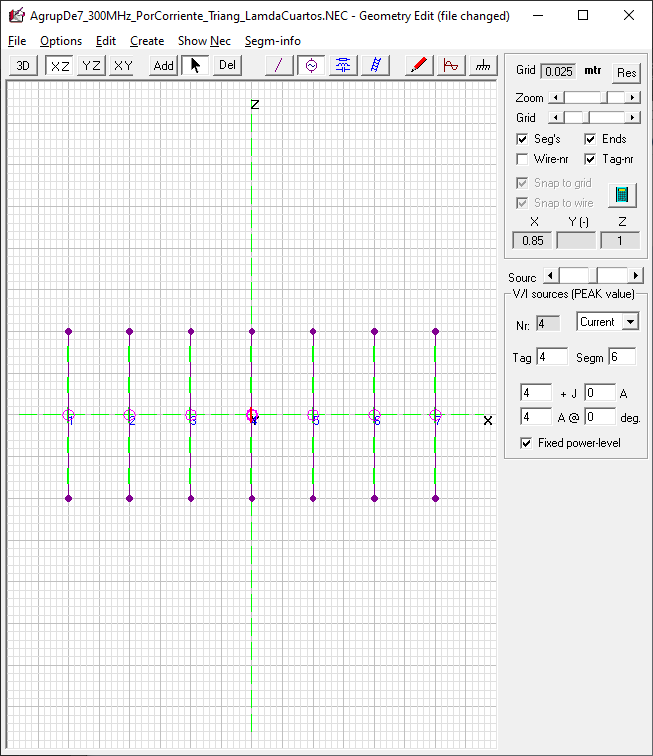
\includegraphics[scale=0.30]{IMAGENES/a52}\label{a52}}	
	\subfloat[]{
		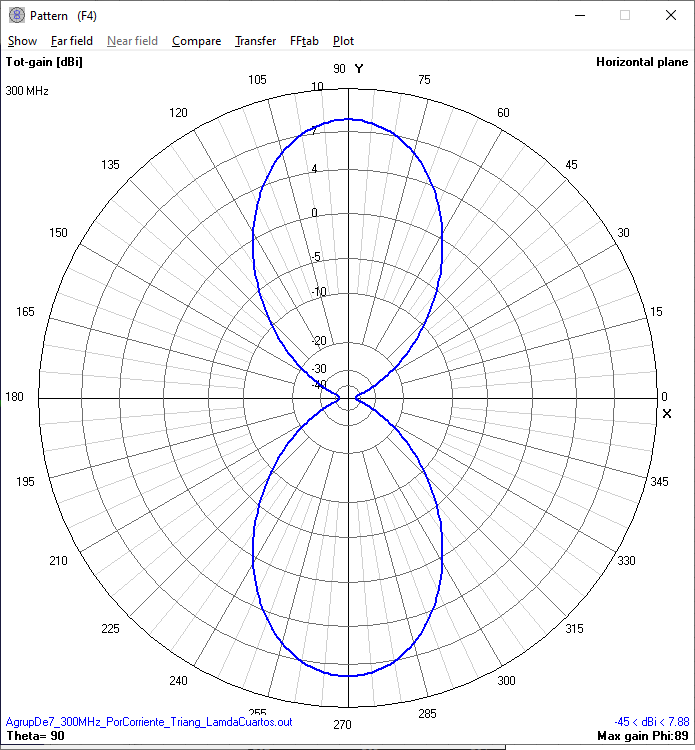
\includegraphics[scale=0.30]{IMAGENES/a53}\label{a53}} \\
	\subfloat[]{
		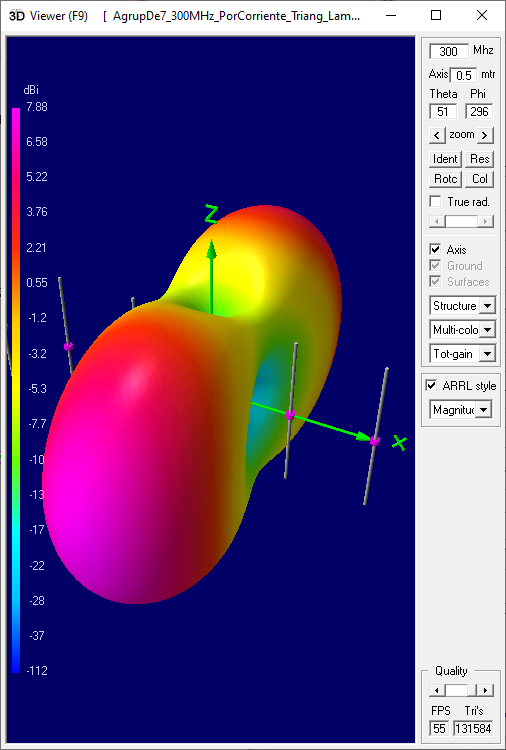
\includegraphics[scale=0.30]{IMAGENES/a54}\label{a54}}
	\subfloat[]{
		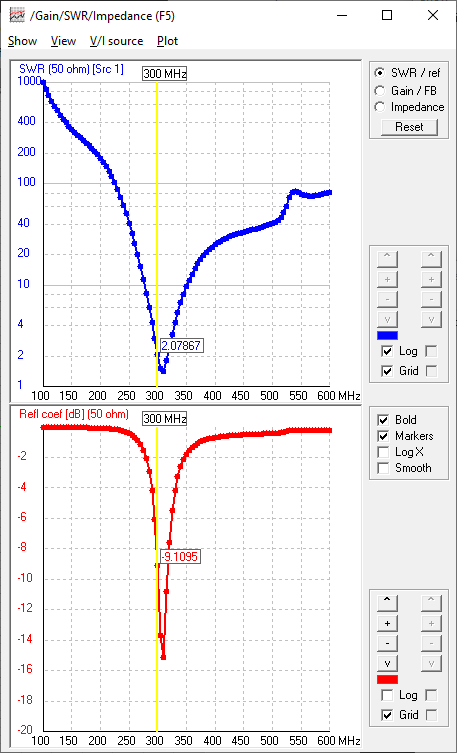
\includegraphics[scale=0.30]{IMAGENES/a55}\label{a55}}
	\caption{(a) Ventana principal para 300MHz, espaciado de $\lambda / 4$ y coeficientes homogeneos. (b) Ventana de edición para ingresar las fuentes homogeneas de acuerdo a los coeficientes. (c) Plano vertical con patrón de radiación. (d) Vista en 3D del patrón de radiación. (e)SWR y coeficiente de refleción.}
\end{figure}

\newpage

\section{Distribución de coeficientes triangular para un espaciado de $\lambda/4$}

Definimos la simulación de las imágenes desde \eqref{a61} hasta \eqref{a65} con los siguientes parámetros:

\begin{align*}
	L = &\lambda/2 =  0.5m \\
	a = & 0.1mm \\
	espaciado = & \lambda / 4 = 0.25m \\
	f = & 300MHz
\end{align*}

Usamos los coeficientes homogeneos de:
\begin{table}[!ht]
	\centering
	\begin{tabular}{c|c|c|c|c|c|c}
		$a_0$ & $a_1$ & $a_2$ & $a_3$ & $a_4$ & $a_5$ & $a_6$ \\ \hline
		1 & 6 & 15 & 20 & 15 & 6 & 1 \\
	\end{tabular}
	\caption{Coeficientes homogéneos}
	\label{tab:6}
\end{table}

Para $f=300MHz$ se obtiene un coeficiente de reflexión de $-3.89dB$ y un SWR de $4.53$. 

\begin{figure}[h]
	\centering
	\subfloat[]{
		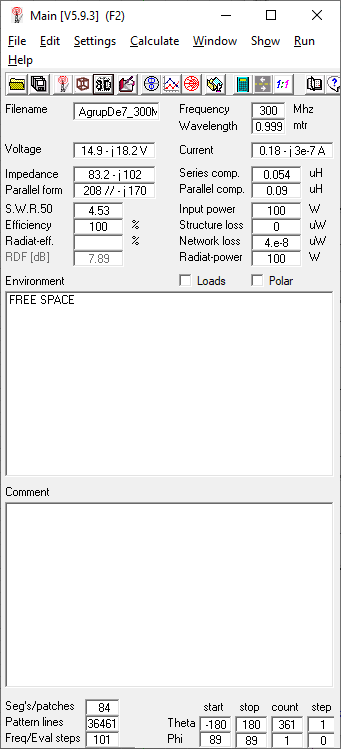
\includegraphics[scale=0.30]{IMAGENES/a61}\label{a61}}
	\subfloat[]{
		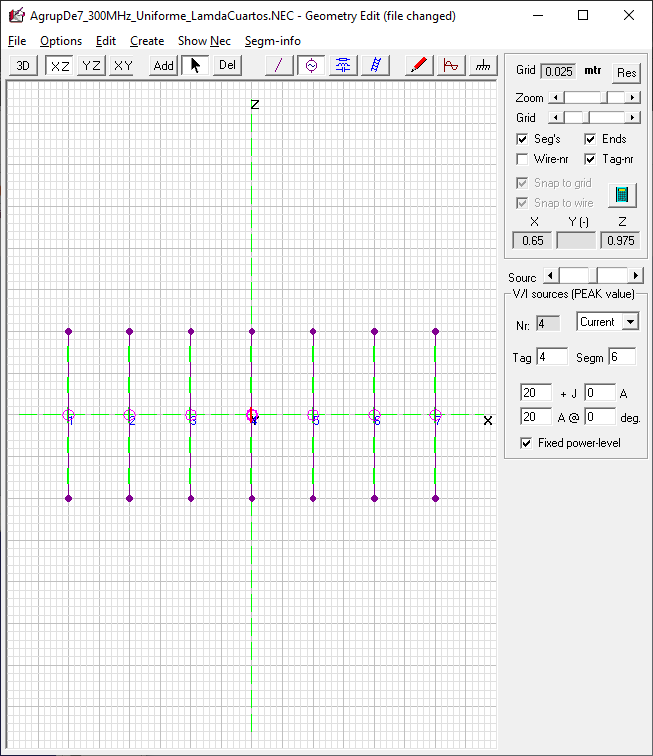
\includegraphics[scale=0.30]{IMAGENES/a62}\label{a62}}	
	\subfloat[]{
		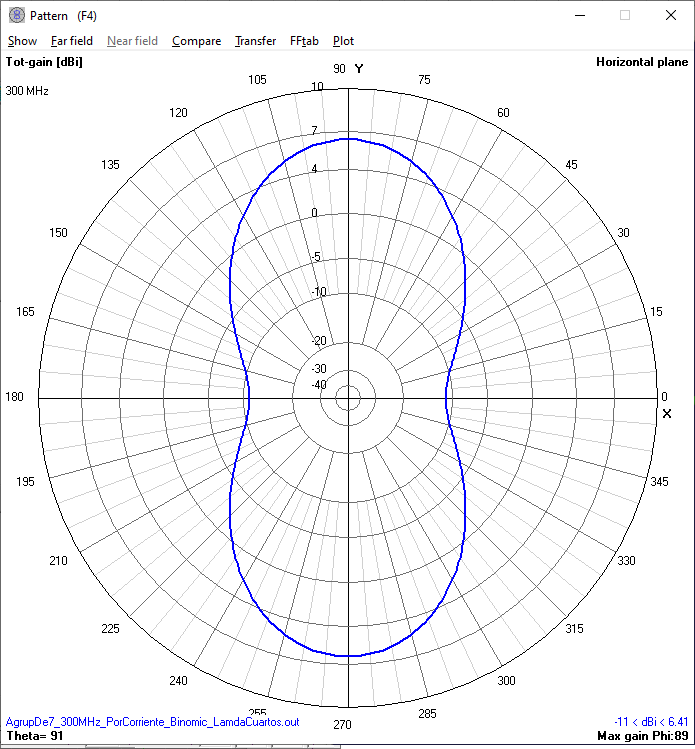
\includegraphics[scale=0.30]{IMAGENES/a63}\label{a63}} \\
	\subfloat[]{
		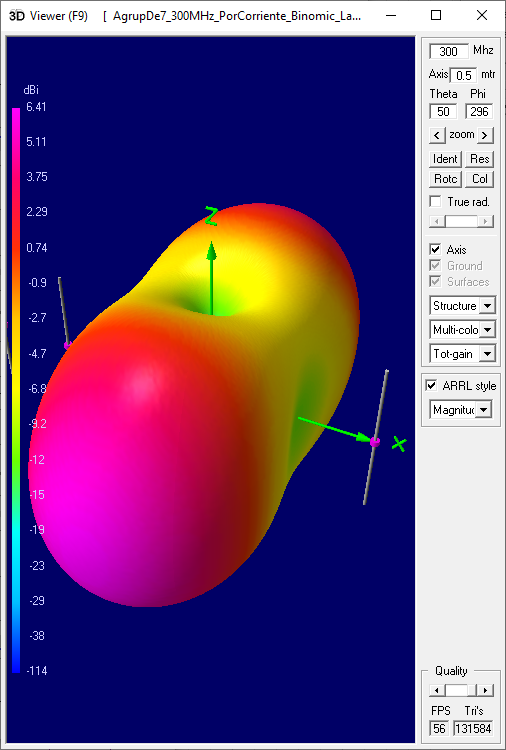
\includegraphics[scale=0.30]{IMAGENES/a64}\label{a64}}
	\subfloat[]{
		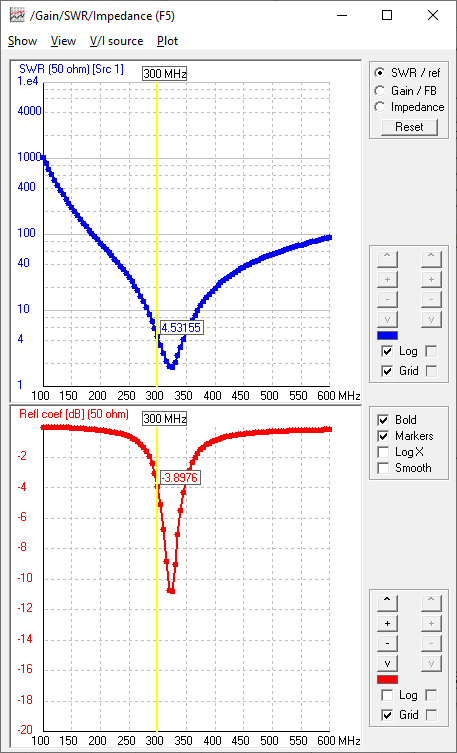
\includegraphics[scale=0.30]{IMAGENES/a65}\label{a65}}
	\caption{(a) Ventana principal para 300MHz, espaciado de $\lambda / 4$ y coeficientes homogeneos. (b) Ventana de edición para ingresar las fuentes homogeneas de acuerdo a los coeficientes. (c) Plano vertical con patrón de radiación. (d) Vista en 3D del patrón de radiación. (e)SWR y coeficiente de refleción.}
\end{figure}

\newpage

\section{Comparación de distribución de coeficientes para un espaciado de $\lambda/4$}

\begin{figure}[h]
	\centering
	\subfloat[]{
		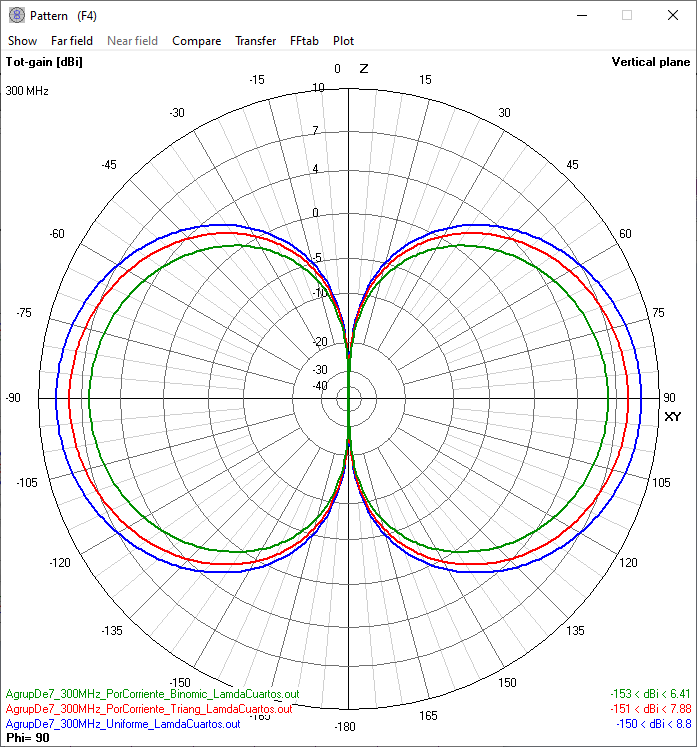
\includegraphics[scale=0.35]{IMAGENES/a444}\label{a333}}
	\subfloat[]{
		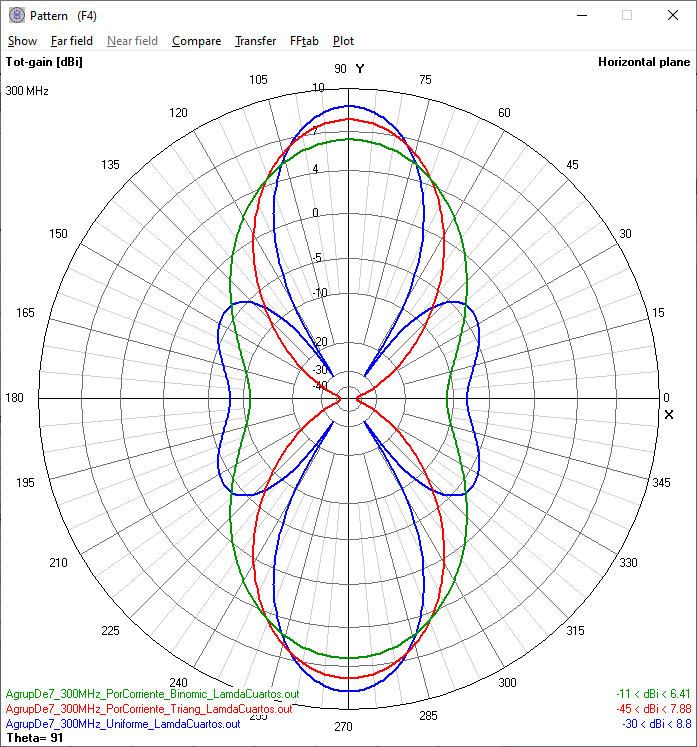
\includegraphics[scale=0.35]{IMAGENES/a333}\label{a444}}	
	\caption{(a) Patrón de radiación horizontal para 300MHz, espaciado de $\lambda / 4$. (b) Patrón de radiación vertical  para 300MHz, espaciado de $\lambda / 4$.  }
\end{figure}

Para una distancia de separación de $\lambda/4 = 0.25$ se tiene dos buenos resultados para diferentes usos. Podemos descartar la distribución homogenea porque tiene lóbulos secundarios muy grandes, a pesar de que cuenta con mejor directividad. 

Para la distribución triangular se tiene un patrón de radiación sin lóbulos secundarios, todo el patrón de radiación se va en su lóbulo principal y posterior. Es muy eficiente y es tan solo un poco menos directivo que con la distribución homogenea. Haciendo algunos rreglos de radio $a$, disminuyendo este radio, o aumentando ligeramente $L$ obtendríamos un coeficiente de radiación a $f=300MHz$. Esta distribución es optima, es bidireccional, un ángulo de haz de 45 grados aproximadamente, y una ganancia máxima de $7.88dBi$. Podría usarse para enlaces no tan lejanos.

Para la distribución binómica se tiene un haz de radiación más abierto con una ganancia máxima de $6.41dBi$. No presenta lóbulos menores, tiene un comportamiento bidireccional y se podría usar para cubrir un area mucho más amplio pero cercano.

\chapter{Concluciones}
Podemos concluir que para una $f=300MHz$ con 7 elementos, podemos ir eliminando lóbulos menores aumentando la corriente de exitación de los elementos centrales (para uso de comportamiento bidireccional). De acuerdo a las districubiones triangular, binómica y homogenea, la que mejor se adecúa para aumentar directividad, es la distribución triangular, ya que a pesar de que puede presentar lóbulos menores, estos son pequeños, incluso desaparecen, como en el caso de un espaciado de $\lambda/4$. Se podría optimizar la directividad y la ganancia, así como el SWR con valores de espaciado entre $\lambda/4$ y $\lambda/2$ usando la distribución triangular.

Pero si queremos cubrir un mayor area, cercana a la vez (bidireccional), y sin pérdida en lóbulos menores, podemos optar por una distribución binómica.

	%----------------------------------------------------------------------------------------
	%	BIBLIOGRAPHY
	%----------------------------------------------------------------------------------------
	
	
	%----------------------------------------------------------------------------------------
	
\end{document}
